\section{Verhaltensspezifikation}

\begin{figure}[H]
    \centering
    \begin{tikzpicture}[]
        % \begin{umlstate}[name=state]{I am a state} 
        % \begin{umlstate}[name=substate1]{I am a substate 1} 
            
        % \end{umlstate} 
        % \begin{umlstate}[x=3, y=-3, name=substate2]{I am a substate 2} 
            
        % \end{umlstate} 
        % \end{umlstate} 
    \end{tikzpicture}
    \caption[Automatengraph Normalbetrieb]{Moore Automatengraph des Normalbetriebs}
    \label{fig:Bild2}
\end{figure}

\begin{figure}[H]
   \centering
   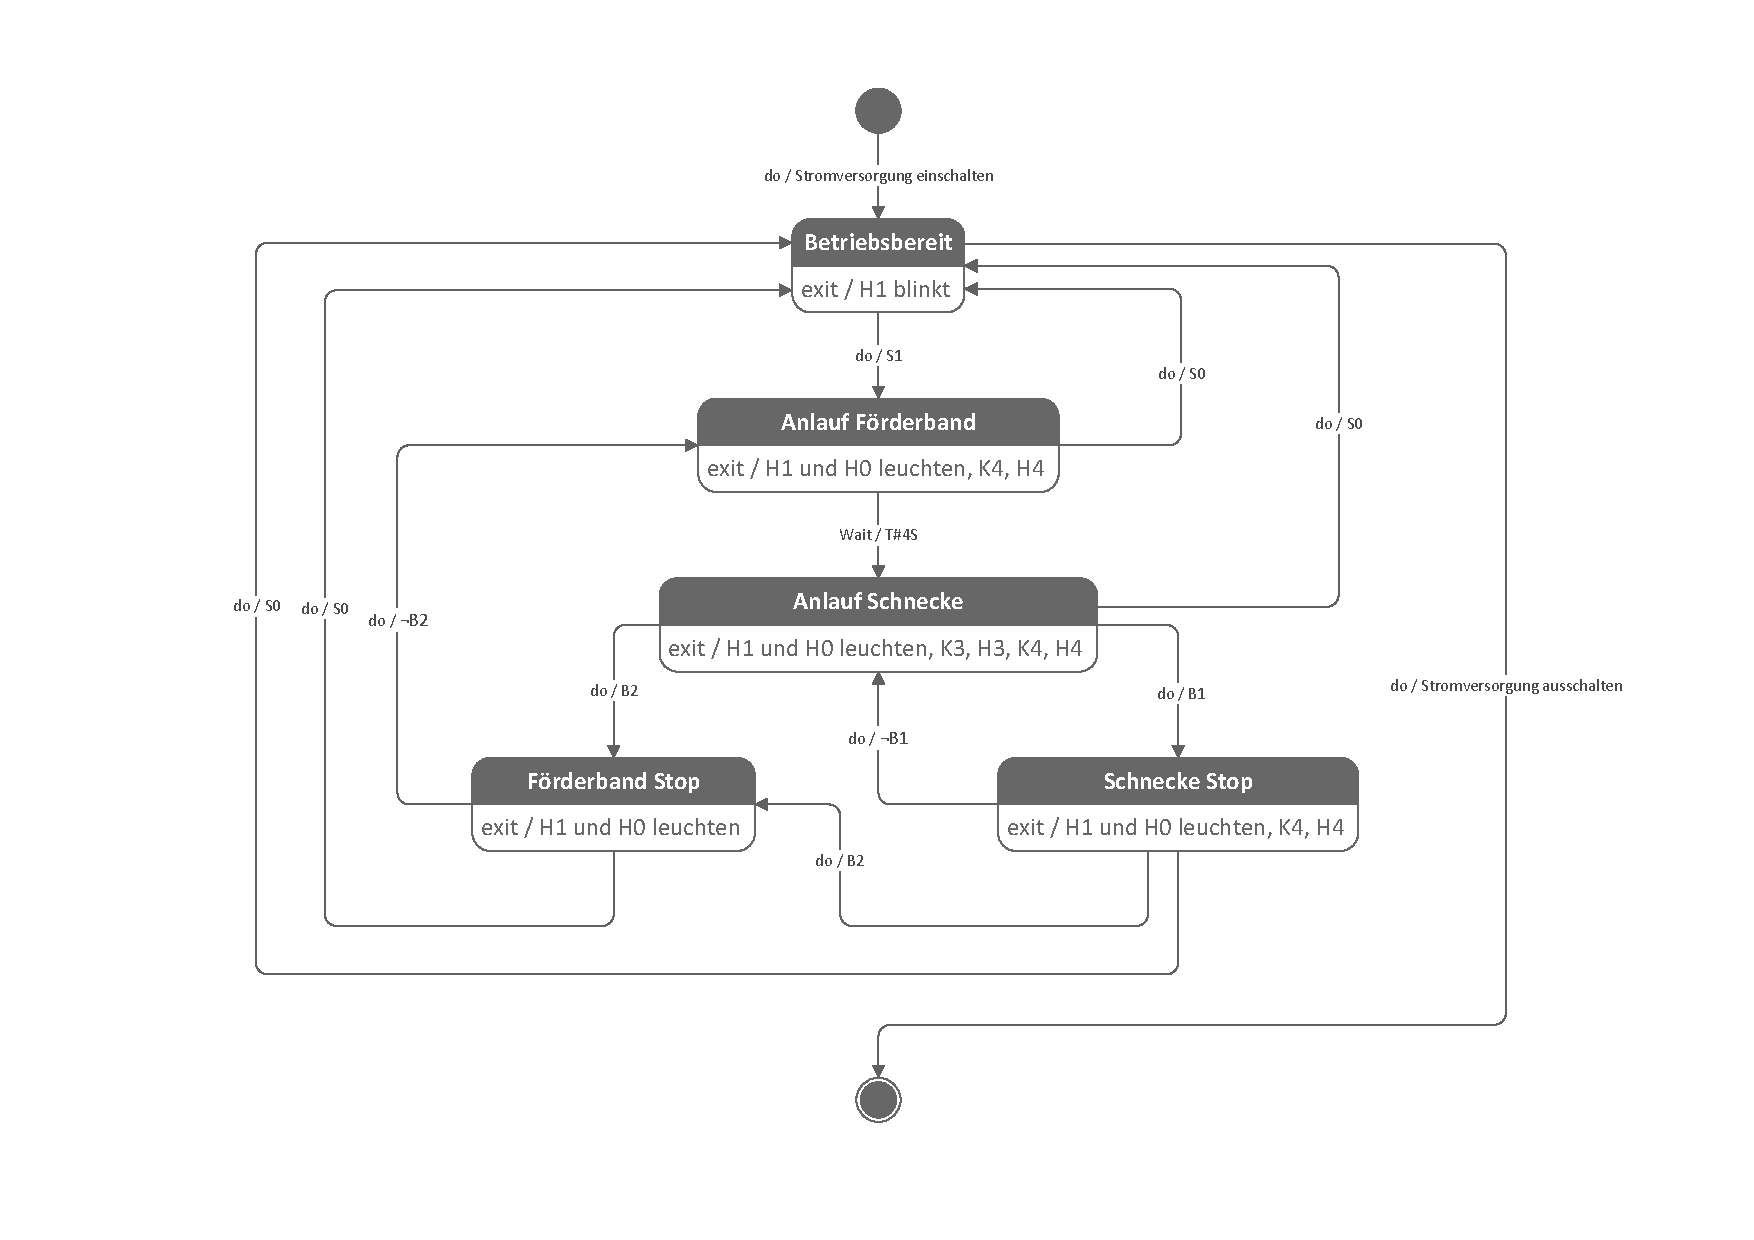
\includegraphics[width=1.0\textwidth]{Bilder/Normalbetrieb.pdf}
   \caption[Automatengraph Normalbetrieb]{Moore Automatengraph des Normalbetriebs (Platzhalter)}
   \label{fig:Bild4}
\end{figure}

\begin{figure}[H]
   \centering
   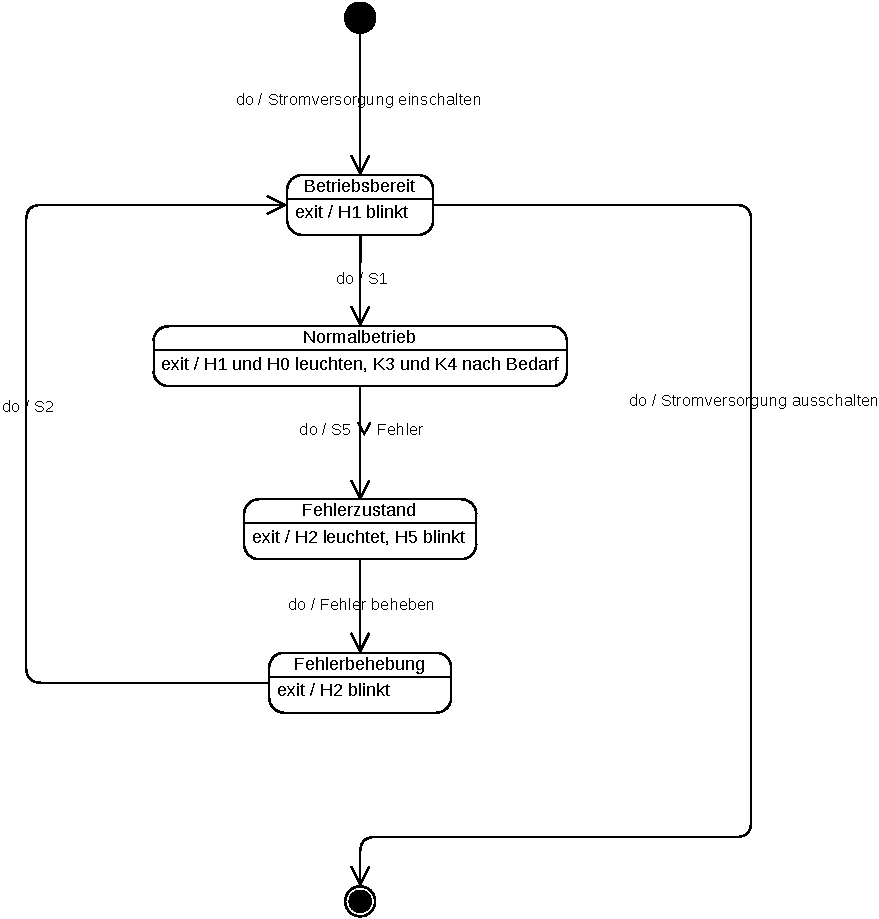
\includegraphics[width=0.8\textwidth]{Bilder/Fehlerfall.pdf}
   \caption[Automatengraph Fehlerfall]{Moore Automatengraph des Fehlerfalls (Platzhalter)}
   \label{fig:Bild5}
\end{figure}